\section{Resultados}
\label{sec:introducao}

Com base nos testes realizados em relação aos resultados das médias de cada inteligência podemos ver que a base Car teve maior acurácia em todas as inteligências exceto pela SVM Learner, o que a torna a melhor base em estudo.

\begin{center}
      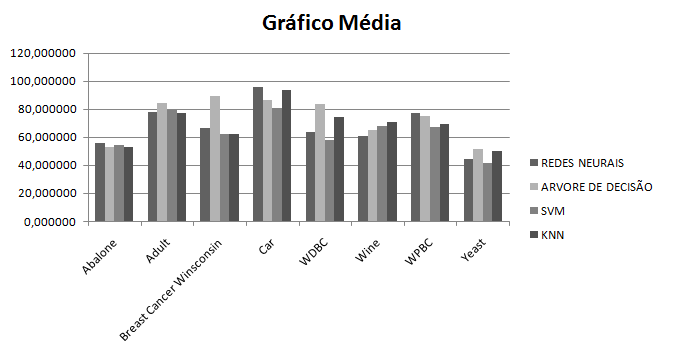
\includegraphics[scale=1.0]{imagens/media.png}
\end{center}

Após a interpretação do gráfico definimos cada base com sua melhor e pior inteligência:

\begin{itemize}
    \item \textbf{Abalone}: A melhor inteligência a ser usada nessa base é a Redes Neurais com 55,68\% enquanto a pior é a KNN com 53,00\%;
    \item \textbf{Adult}: A melhor inteligência a ser usada nessa base é a Árvore de Decisão com 84,51\% enquanto a pior é a KNN com 76,96\%;
    \item \textbf{Breast Cancer Winsconsin}: A melhor inteligência a ser usada nessa base é a Árvore de Decisao com 89,46\% enquanto a pior é a KNN com 62,05\%;
    \item \textbf{Car}: A melhor inteligência a ser usada nessa base é a Redes Neurais com 95,73\% enquanto a pior é a SVM com 80,76\%;
    \item \textbf{WDBC}: A melhor inteligência a ser usada nessa base é a Árvore de Decisão com 83,27\% enquanto a pior é a SVM com 57,94\%;
    \item \textbf{Wine}: A melhor inteligência a ser usada nessa base é a KNN com 70,69\% enquanto a pior é a Redes Neurais com 60,60\%;
    \item \textbf{WPBC}: A melhor inteligência a ser usada nessa base é a Redes Neurais com 77,23\% enquanto a pior é a SVM com 69,51\%;
    \item \textbf{Abalone}: A melhor inteligência a ser usada nessa base é a Árvore de Decisão com 51,21\% enquanto a pior é a SVM com 41,74\%.
\end{itemize}